%%%%%%%%%%%%%%%%%%%%%%%%%%%%%%%%%%%%%%%%%%%%%%%%%%%%%%%%%%%%%%%%%%%%%%%%%%%%%%%
%                                                                             %
% 01 - Introducción y objetivos                                               %
%                                                                             %
%%%%%%%%%%%%%%%%%%%%%%%%%%%%%%%%%%%%%%%%%%%%%%%%%%%%%%%%%%%%%%%%%%%%%%%%%%%%%%%

\chapter{\textcolor{azulescom}{Introducción}}


\section{SkyPrice}

% Imagen con el logo de SkyPrice
\begin{figure}[H]
  \centering
  
\includegraphics[width=0.2\textwidth]{imagenes/01-introduccion/skyprice-logo.png}
  \caption{Logo de SkyPrice}
  \label{fig:skyprice-logo}
\end{figure}

\textit{SkyPrice} es una aplicación web que permite a los usuarios realizar estimaciones
de precios de mercado para departamentos en la Ciudad de México. La aplicación
utiliza tres modelos de \textit{machine learning} estimar el precio de un departamento
dado un conjunto de características. Además, \textit{SkyPrice} permite a los
usuarios visualizar los datos de entrenamiento así como otros conjuntos de datos
relevantes a la Ciudad de México en un mapa interactivo. Se provee una API pública
para aquellos usuarios interesados en integrar la funcionalidad de estimación de precio
en sus propios proyectos y, también se incluye
una sección con información detallada del proyecto.

\section{Propósito de este manual de usuario}

Este manual de usuario tiene como objetivo proporcionar a los usuarios de \textit{SkyPrice}
una guía detallada sobre cómo utilizar la aplicación web. En este manual, los usuarios
encontrarán información sobre cómo acceder a la aplicación, cómo realizar estimaciones
de precios de mercado para departamentos y cómo visualizar un mapa interactivo con los
anuncios de departamentos en la Ciudad de México.

\section{¿Cómo usar este manual?}
Este manual está organizado en función de las pantallas y funcionalidades de la
aplicación web. En el capítulo dos, se describen los requerimientos y cómo acceder
a la aplicación web. En el capítulo tres, se explica cómo realizar estimaciones de
precios de mercado para departamentos. En el capítulo cuatro, se detalla cómo visualizar
información sobre los modelos y detalles de los datos. El quinto capítulo está
dedicado al mapa interactivo y los conjuntos de datos disponibles. En el capítulo
seis, se discute la funcionalidad de API pública para aquellos usuarios
interesados en acceder a documentación especializada. Finalmente, en el capítulo
siete, se presentan las conclusiones y recomendaciones finales.

\section{Idiomas disponibles}
SkyPrice está pensado para ser accesible a un público amplio, por lo que la aplicación
está disponible en los siguientes idiomas:

\begin{itemize}
  \item Español
  \item Inglés
  \item Francés
  \item Portugués
\end{itemize}

Para cambiar el idioma de la aplicación, los usuarios pueden seleccionar el idioma
deseado desde la barra de navegación, accesible en la parte superior de la página.
En la figura \ref{fig:idiomas-disponibles} se muestra un ejemplo de cómo cambiar el idiomas
de la aplicación.

% Imagen con los idiomas disponibles
\begin{figure}[H]
  \centering
  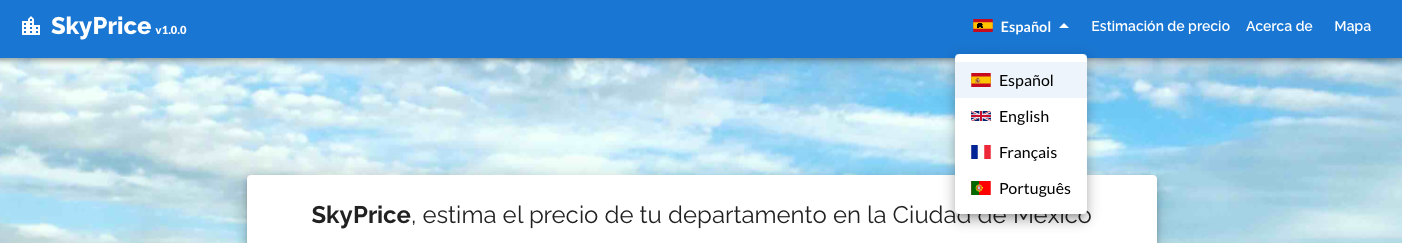
\includegraphics[width=1.0\textwidth]{imagenes/01-introduccion/traducciones.png}
  \caption{Idiomas disponibles en SkyPrice}
  \label{fig:idiomas-disponibles}
\end{figure}

